\chapter{Vorbereitung}

\section{Das Drude-Modell}

Die von P. Drude um 1900 entwickelte Theorie zur Leitfähigkeit in Metallen stellte
einen Sprung im Verständnis der Elektronenbewegungen dar. Wesentliche Ergebnisse
dieser Betrachtung sind die Driftgeschwindigkeit $v_{d}$, die mittlere Stoßzeit
$\tau$ und die klassische Bewegungsgleichung für Elektronen dar. Diese Ergebnisse
werden auch zur Erklärung des klassischen Hall-Effekts benötigt. Deshalb soll nun
ein kurzer Überblick gegeben werden.\\\\
Die Theorie beschreibt Bewegungen von Elektronen in Leitern durch die kinetische
Gastheorie. Diese werden als freie Teilchen mit der thermischen Geschwindigkeit
$v_{th}$ betrachtet, die mit Atomrümpfen stoßen. Die zugehörige Bewegungsgleichung:
\[
    m \dot{\vec{v}} = - e \vec{E} - m \frac{v_{d}}{\tau}
\]
Die Driftgeschwindigkeit $v_{d}$ bezeichnet die vom E-Feld bewirkte zusätzliche 
Geschwindigkeit $(v-v_{th})$. Die Relaxationszeit $\tau$ die Zeit, nach welcher die
Driftgeschwindigkeit nach Abschalten des Feldes in den Gleichgewichtszustand geht,
also $v_{d} = 0$. Dieser Wert ist charakteristisch für jedes Material und muss
experimentell bestimmt werden. Der ganze Term $ m \, \vec{v_{d}} / \tau$ beschreibt
eine Reibungs- oder Dämpfkraft. Im Modell wird die hemmende Wirkung der Stöße durch
diesen berücksichtigt. Der Term $-e \vec{E}$ beschreibt die durch das elektrische 
Gleichfeld auf die Elektronen wirkende konstante Kraft.\\\\
Im stationären Fall, also $\dot{\vec{v}} = 0$, ergibt sich:
\[
    v_{d} = \frac{-e \tau}{m} \vec{E} = - \mu \vec{E}
\]
mit der Beweglichkeit $\mu = e \tau / m$. Für die Stromdichte kann man errechnen:
\[
    \vec{j} = -en\vec{v_{d}} = \frac{ne^{2}\tau}{m} \vec{E} = ne \mu \vec{E}
\]
Hier bezeichnet $n$ die Elektronendichte. Weiter folgt für die Leitfähigkeit:
\[
    \sigma = \frac{j}{E} = \frac{ne^{2}\tau}{m} = ne \mu
\]
Somit ist Drude gelung das Ohm'sche Gesetz auf zwei Materialparameter
zurückzuführen.\\\\

Es gilt zu beachten, dass dieses Modell annimmt, alle Leitungselektronen würden
beschleunigt und gestreut. Dies ist jedoch mit dem Resultat unverträglich, dass
Elektronen der Fermi-Dirac-Statistik unterliegen. Genauere Modelle kamen für diesen
Fall später jedoch auf das gleiche Ergebnis, sodass diese Betrachtung für die 
Erklärung des klassischen Hall-Effekt ausreicht. \cite{hunklinger}

\section{Der klassische Hall-Effekt}

Der klassische Hall-Effekt beschreibt den Effekt eines Magnetfeldes auf eine
Probe. So baut sich im Inneren der Probe ein elektrisches Feld auf, dessen
resultierende elektrische Kraft im stationären Zustand gerade die Lorentz-Kraft
kompensiert.\\
Zur Diskussion beginnt man mit der klassischen Bewegungsgleichung im Magnetfeld:
\[
    m^* \dot{\vec{v}} = - e \left( \vec{E} + \vec{v}_d \times \vec{B} \right)
                      - m^* \frac{\vec{v}_d}{\tau}
\]
Hierbei sind $\vec{v}_d$, $\tau$ und $\vec{E}$ aus dem Drude-Modell bekannt.
$m^*$ bezeichnet die effektive Masse und $\vec{B}$ das Magnetfeld. 
Da die Elektronen bei jedem Stoß ihre Bewegungsrichtung ändern, bleibt außerdem
nur der durch die Driftgeschwindigkeit verursachte Beitrag 
$-e \left( \vec{v}_d \times \vec{B} \right)$ übrig.\\
Zur Vereinfachung betrachten wir ein in $z$-Richtung anliegendes Magnetfeld
im stationären Fall, also $\dot{\vec{v}} = 0$. Somit ergibt sich:
\begin{align*}
    \vec{v}_{d,x} &= - \frac{e \tau}{m^*} \left( E_x + \vec{v}_{d,y} \; B \right),\\
    \vec{v}_{d,y} &= - \frac{e \tau}{m^*} \left( E_y + \vec{v}_{d,x} \; B \right),\\
    \vec{v}_{d,x} &= - \frac{e \tau}{m^*} E_z
\end{align*}
Mit der Elektronendichte
\[
    j = -e n \vec{v}_d = \frac{n e^2 \tau}{m} \vec{E} = n e \mu E
\]
aus der für die elektrische Leitfähigkeit folgt
\[
    \sigma = \frac{j}{E} = \frac{n e^2 \tau}{m} = n e \mu
\]
folgt für die Stromdichte im betrachteten Fall:
\[
    \begin{pmatrix}
        j_x\\ j_y \\ j_z
    \end{pmatrix} 
    = - \frac{\sigma_0}{1 + \omega_c^2 \tau^2}
      \begin{pmatrix}
          1             & -\omega_c \tau    & 0 \\
          \omega_c \tau & 1                 & 0 \\
          0             & 0                 & 1+\omega_c^2 \tau^2 \\
      \end{pmatrix}
      \begin{pmatrix}
          E_x \\ E_y \\ E_z
      \end{pmatrix}
\]
Hier bezeichnet $\omega_0 = n e^2 \tau / m^*$ die Leitfähigkeit ohne Magnetfeld
und $\omega_c$ für die Zyklotronfrequenz.\\
Zur Vereinfachung betrachten wir einen flachen Stab mit rechteckigen Querschnitt.
Der Strom fließt hierbei in $x$-Richtung. Mit dieser Geometrie tritt in
$z$-Richtung kein elektrisches Feld auf. Somit vereinfacht sich obiger Ausdruck zu:
\[
    \begin{pmatrix}
        j_x \\ j_y
    \end{pmatrix}
    = \begin{pmatrix}
         \omega_{xx} & \omega_{xy} \\
        -\omega_{xy} & \omega_{xx}
      \end{pmatrix}
      \begin{pmatrix}
          E_x \\ E_y
      \end{pmatrix}
\]
Hier wurden die Leitwerte
\[
    \omega_{xx} = \frac{ne}{B} \frac{\omega_c \tau}{1+\omega_c^2 \tau^2}, \qquad
    \omega_{xy} = -\frac{ne}{B} \frac{\omega_c^2 \tau^2}{1+\omega_c^2 \tau^2}
\]
eingeführt.\\
Löst man das Gleichungssystem nach den elektrischen Feldern auf erhält man:
\[
    \begin{pmatrix} E_x \\ E_y \end{pmatrix}
    = \begin{pmatrix}
         \rho_{xx} & \rho_{xy} \\
        -\rho_{xy} & \rho_{xx} 
      \end{pmatrix}
      \begin{pmatrix}
          j_x \\ j_y
      \end{pmatrix}
\]
mit den spezifischen Widerständen:
\[
    \rho_{xx} = \frac{B}{ne} \frac{1}{\omega_c \tau} = \frac{m^*}{ne^2\tau}, \qquad
    \rho_{xy} = \frac{B}{ne}
\]
Hier wird $\rho_{xx}$ als Längswiderstand $R$ und $\rho_{xy}$ als Hall-Widerstand
$R_H$ bezeichnet.
In einem anisotropen Medium würden die Größen $\rho_{yx}$ und $\rho_{yy}$
auftreten. Für isotrope Medien, die hier betrachtet werden sollen, gilt jedoch:
$\rho_{xx} = \rho_{yy}$ und $\rho_{yx} = - \rho_{xy}$. Ein Plot der klassischen
Widerstände ist in Abbildung \ref{Abb:klassisch} zu sehen. \cite{hunklinger}
\begin{figure}
    \centering
        \begin{subfigure}[c]{0.45\textwidth}
        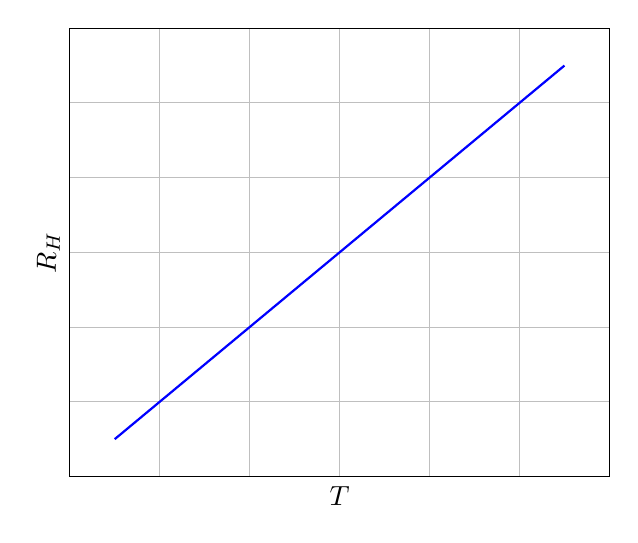
\begin{tikzpicture}
            \begin{axis}[
                ticks=none,
                xlabel={$T$}, ylabel={$R_H$},
                grid=both
            ]
                \addplot[thick, blue] {x};
            \end{axis}
        \end{tikzpicture}
        \caption{Hall-Widerstand}
    \end{subfigure}
    \begin{subfigure}[c]{0.45\textwidth}
        \begin{tikzpicture}
            \begin{axis}[
                ticks=none,
                xlabel={$T$}, ylabel={$R_\square$},
                grid=both
            ]
                \addplot[thick, blue] {1};
            \end{axis}
        \end{tikzpicture}
        \caption{Schichtwiderstand}
    \end{subfigure}

    \caption{Widerstände beim klassischen Hall-Effekt}
    \label{Abb:klassisch}
\end{figure}

\section{Quanten-Hall-Effekt}
\subsection{Zweidimensionales Elektronengas}

Die Untersuchung des Quanten-Hall-Effekts wird an einem sog. zweidimensionalen
Elektronengas durchgeführt. Hierbei handelt es sich um ein freies Elektronengas, 
also die Elektronen können sich näherungsweise frei in alle Raumrichtungen bewegen,
dass in einer Raumrichtung durch einen schmalen Potentialtopf eingeschränkt wird.
Dies führt zu einer Quantisierung der Gesamtenergien, die ein Elektron haben kann.
Ist nun nur das unterste Niveau besetzt, so können sich die Teilchen in zwei 
Richtungen frei bewegen, während sie in die dritte eingesperrt sind. Somit ergibt
sich der Begriff des Zweidimensionales Elektronengases.\\\\
Zur theoretischen Betrachtung wählt man den Potentialtopf zur Vereinfachung in 
$z$-Richtung. Die Energie in z-Richtung ist somit quantisiert und darstellbar als
$E_{s} (s=0,1,\dots)$. Für die Gesamtenergie eines Elektrons ergibt sich:
\[
	E(s,k_{x},k_{y}) = E_{s} + \frac{\hbar^{2} k_{x}^{2}}{2m^{*}}
					   + \frac{\hbar^{2} k_{y}^{2}}{2m^{*}}, \qquad{}
	(s=0,1,\dots)
\]
$E_{s}$ ist unabhängig vom Wellenvektor $\vec{k}$, da in $z$-Richtung keine 
Bewegung stattfindet. Die beiden hinteren Terme beschreiben die kontinuierliche
freie Bewegung in der $x-y$-Ebene. $m^{*}$ bezeichnet die effektive Masse.

\subsection{Theorie des Quanten-Hall-Effekt}

Misst man den Hall-Effekt nun an einem Zweidimensionalen Elektronengas bei wenigen
Kelvin und Magnetfeldern im einstelligen Teslabereich, so weicht das Ergebnis vom
klassischen Hall-Effekt ab. Ein Beispiel dafür ist in Abbildung \ref{Abb:qhe} 
dargestellt.

\begin{figure}[ht]
    \centering
    \def\svgwidth{0.6\linewidth}
    \import{Abb/}{quanten_hall.pdf_tex}
    \caption{Hall und Schichtwiderstand beim Quanten-Hall-Effekt \cite{nobelqhe}}
    \label{Abb:qhe}
\end{figure}

Bei kleinem Magnetfeld deckt sich der Graph mit dem linearen Anstieg beim
klassischen Hall-Effekt. Bei größeren Feldern bilden sich Plateaus bei bestimmten 
Widerstandswerten aus:
\[
	R_{H} = \frac{1}{\nu} \frac{\hbar}{e^{2}}, \qquad (\nu=1,2,\dots)
\]
Dies wird als Quanten-Hall-Effekt bezeichnet.
Gleichzeitig oszilliert der Längswiderstand bei hohen Feldstärken. Die wirkliche
ist jedoch sehr viel kleiner als der Hall-Widerstand. In Abbildung \ref{Abb:qhe}
wurden deshalb beide Werte normalisiert, um die Lesbarkeit zu verbessern. 
Die Minima der Oszillationen, bei denen der Längswiderstand verschwindet, liegt auf
den Plateaus des Hall-Widerstands. Dieses Phänomen wird als
Shubnikov-de-Haas-Oszillation bezeichnet.\\\\
Zur theoretischen Betrachtung stellt man folgende Schrödingergleichung auf:
\[
	\left(
		\frac{( i\hbar\nabla+e \, \vec{A}(x,y) )^{2}}{2m^{*}} + U(y)
	\right) \Psi(x,y) = E \, \Psi(x,y)
\]
Hier wählt man $\vec{A} = (-By,0,0)$, sodass $\vec{B} = rot \vec{A}$ in $z$-Richtung
zeigt. Das Randpotential $U(y)$ schränkt die Elektronenbewegung auf die Ausdehnung
der Probe ein.
Weiter wird nun eine eine ausreichend große Probe angenommen, sodass $U(y)$ 
vernachlässigt werden kann:
\newcommand{\zweim}{\frac{1}{2m^{*}}}
\[{}
	\zweim \left( (p_{x} + e B y)^{2} + p_{y}^{2}\right) \Psi(x,y) = E \Psi(x,y)
\]
$p_{x} = - i \hbar \partial_{x}$ und $p_{y} = - i \hbar \partial_{y}$ bezeichnen die
Impulsoperatoren in $x$- bzw. $y$-Richtung.
Zur Lösung wird nun der Separationsansatz verwendet:
\[
	\Psi(x,y) = \phi(x) \chi(y) = \frac{1}{\sqrt{L}} \exp(ikx) \chi(y)
\]
Für $\chi(y)$ muss also gelten:
\[
	\zweim \left[ (\hbar k + eBy)^{2} + p_{y}^{2} \right] \chi(y) = E \chi(y)
\]
Diese Gleichung kann in die Schrödingergleichung eines eindimensionalen,
harmonischen Oszillators umgeformt werden. Hierzu wird die Frequenz
$\omega_{c} = \frac{e B}{m^{*}}$ und die Zentrumskoordinate 
$y_{k} = \frac{\hbar k}{eB}$ eingeführt. Durch einfaches Einsetzen ergibt sich:
\[
	\left[ \frac{p_{y}^{2}}{2m^{*}} + \frac{1}{2} m^{*} \omega_{c}^{2}
	(y + y_{k})^{2} \right] \chi(y) = E \chi(y)
\]
Die Frequenz des harmonischen Oszillators ist die eingeführte Frequenz $\omega_{c}$.
Die Koordinate $y_{k}$ bezeichnet die Verschiebung des harmonischen Oszillators auf
der $y$-Achse vom Nullpunkt.\\\\
Die Eigenfunktionen haben die Form:
\begin{align*}
    &\chi_{n,k}(y) = \exp \left[ - \frac{(q+q_{k})^{2}}{2} \right]
                    H_{n} (q+q_{k})\\
    &q = \sqrt{\frac{m^{*} \omega_{c}}{\hbar}} y, \qquad 
     q_{k} = \sqrt{\frac{m^{*}\omega_{c}}{\hbar}}y_{k}
\end{align*}
$H_{n}$ bezeichnet das n-te Hermitesche Polynom. Für das weitere Vorgehen betrachtet
man die Energiewerte, die unabhängig von $k$ sind und diskrete Werte annehmen:
\[
    E_{n} = \left(n + \frac{1}{2}\right) \hbar \omega_{c}
    \qquad (n=0,1,2,\dots)
\]
Dies sind die Energiewerte der sogenannten Landauniveaus. 

\begin{figure}
    \centering
        % Parabel
    \begin{subfigure}[c]{0.33\textwidth}
    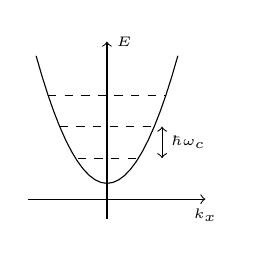
\begin{tikzpicture}
        % Koordinatensystem
        \draw [->] (0,-0.25) -- (0,2);
        \draw [->] (-1,0) -- (1.25,0);
        \draw (0,2) node[anchor=west] {\tiny $E$};
        \draw (1.25,0) node[anchor=north] {\tiny $k_x$};
        % Funktion
        \draw[domain=-0.9:0.9] plot ({\x}, {2*\x*\x+0.2});
        % Beschriftung
        \draw [dashed] (-0.37,0.52) -- (0.4,0.52);
        \draw [dashed] (-0.6, 0.92) -- (0.6,0.92);
        \draw [dashed] (-0.748,1.32) --(0.748,1.32);
        \draw [<->] (0.7,0.52) -- (0.7,0.92);
        \draw (0.7,0.72) node[anchor=west] {\tiny $\hbar \omega_c$};
    \end{tikzpicture}
    \caption{Diskrete Zustände bei Energiewerte, der Landauniveaus}
    \end{subfigure}
    % Kreise
    \begin{subfigure}[c]{0.33\textwidth}
    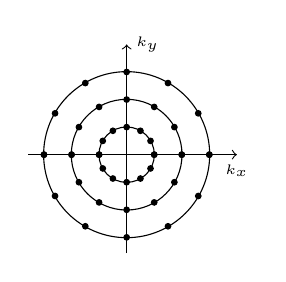
\begin{tikzpicture}
        % Koordinatensystem
        \draw [->] (-1.25,0) -- (1.4,0);
        \draw [->] (0,-1.25) -- (0,1.4);
        \draw (1.4,0) node[anchor=north] {\tiny $k_x$};
        \draw (0,1.4) node[anchor=west] {\tiny $k_y$};
        % Kreise
        \draw (0,0) circle (10pt);
        \draw (0,0) circle (20pt);
        \draw (0,0) circle (30pt);
        % Zustände
        \foreach \r in {0.35,0.7,1.05}{
            \foreach \x/\y in {0/1,1/0,-1/0,
                               0.8660254037844387/0.49999999999999994,% pi/6
                               0.49999999999999994/0.8660254037844387,% pi/3
                               -0.4999999999999998/0.8660254037844387,
                               -0.8660254037844387/0.49999999999999994
            }{
                \pgfmathsetmacro{\test}{1-(\x*\x)}
                \draw [fill] (\r*\x,\r*\y) circle (1pt);
                \draw [fill] (\r*\x,-\r*\y) circle (1pt);
            }
        }
    \end{tikzpicture}
    \caption{Zustände kondensieren auf Kreislinien}
    \end{subfigure}
    % Energiediagramm
    \begin{subfigure}[c]{0.3\textwidth}
        \begin{tikzpicture}[scale=1.2]
            \begin{axis}[xmin=0,xmax=4.5,ymax=1.2,
                xlabel={$E$},ylabel={$D(E)$},
                x label style={at={(current axis.right of origin)},
                               anchor=north,below=-0mm,left=-0.5mm},
                y label style={at={(current axis.above origin)},
                               anchor=south,below=-2mm},
                ticks=none]
                \addplot[blue] coordinates {(1,0)(1.1,1)(1.2,0)} ;
                \addplot[blue] coordinates {(2,0)(2.1,1)(2.2,0)} ;
                \addplot[blue] coordinates {(3,0)(3.1,1)(3.2,0)} ;
            \end{axis}
            \draw [<->] (0.8,0.95) -- (1.1,0.95);
            \draw (0.95,0.95) node[anchor=south] {\tiny $\hbar \omega_c$};
        \end{tikzpicture}
    \caption{Zustandsdichte spaltet in diskrete Landauniveaus auf}
    \end{subfigure}

    \caption{Energiezustände in verschiedenen Darstellungen: Beim Anlegen eines
             Magnetfeldes gibt es nur diskrete Zustände, die besetzt werden können.}
    \label{fig:landau}
\end{figure}

    \subsection{Herstellung eines Zweidimensionalen Elektronengases}
    Die Realisierung eines zweidimensionalen Elektronengases (2DEG) erfolgt bei
    unserem Versuch an der Grenzfläche zweier verschiedener Halbleitermaterialien:
    mit Silizium dotiertes AlGaAs besitzt eine energetisch höheres Leitungsband
    als GaAs, weswegen Elektronen in Richtung GaAs fließen. Durch diese
    Ladungsverschiebung werden die verschieden Ferminiveaus der Schichten
    angeglichen, sowie die Valenz- und Leitungsbänder verzerrt, wodurch eine Art
    Potentialtopf in der Grenzfläche entsteht. Um die Elektronen in diesem
    Potentialtopf von Wechselwirkungen mit den Donatoren in der Dotierschicht
    abzuschirmen, wird noch eine sog. Spacerschicht dazwischen geschoben.
    Diese besteht aus undotiertem AlGaAs. Außerdem wird noch eine Deckschicht
    aus GaAs aufgewachsen, welche nur als Oxidationsschutz dient und für die
    Erzeugung des 2DEG sonst von keiner Bedeutung ist. Die Schichtfolge mit den
    dazugehörigen Bandstrukturen und dem Potentialtopf ist in Abb. dargestellt.

\begin{figure}[H]
	\centering
	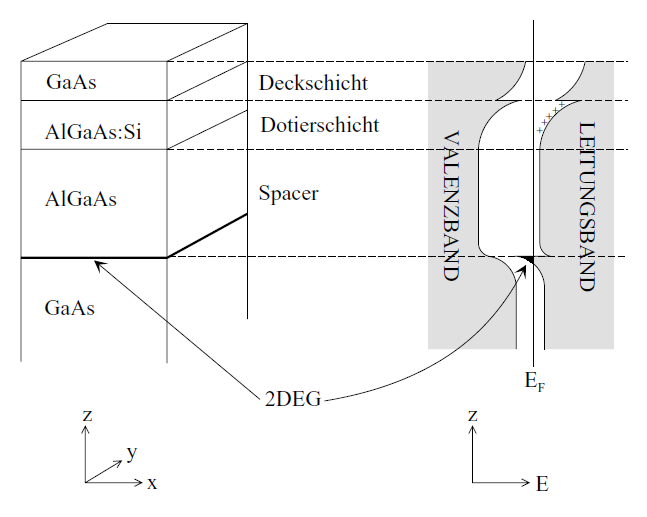
\includegraphics[width=0.75\linewidth]{Abb/Schichtfolge.PNG}
	\caption{Schematische Darstellung der Schichtfolge mit Bandstruktur. Die Bänder sind durch die Ladungsverschiebung verzerrt und an der Grenzschicht von AlGaAs zu GaAs entsteht ein Potentialtopf (schwarz).}
\end{figure}

	\subsection{Van-der-Pauw-Methode}
	Die Van-der-Pauw-Methode beschreibt ein Messverfahren, das ohne die äußerst aufwendige Herstellung einer Hallgeometrie in einer Halbleiterstruktur auskommt. Kurz zusammengefasst wird der Widerstand der Probe durch systematisches Vertauschen der Kontakte bestimmt. Dadurch ist die Geometrie der Probe bei diesem Verfahren nahezu beliebig und auch die Platzierung der Messkontakte muss nicht so präzise erfolgen, was einen deutlich einfacheren Messaufbau erlaubt.
	
	Eine Van-der-Pauw-Geometrie bezeichnet ein Halbleiterstück, welches mit vier Kontakten (im Folgenden jeweils mit A,B,C und D bezeichnet) versehen ist. Dabei wird davon ausgegangen, dass die Kontakte klein sind und sich am Rand der Probe befinden. Zudem muss die Halbleiterprobe homogen und gleichmäßig dotiert sein, sowie keine Löcher aufweisen. Es ist für die Messgenauigkeit jedoch von Vorteil eine möglichst symmetrische Probengeometrie zu wählen; also beispielsweise - wie in diesem Versuch - eine quadratische Form mit den Kontakten an den Ecken (siehe auch Abb.\ref{vdP}).
	
	Bei der Messung wird folgendermaßen vorgegangen: zwischen zwei Kontakten wird die Spannung gemessen, während durch die beiden anderen Kontakte ein Strom geschickt wird. Der zu dieser Messung gehörige Widerstand wird dann mit \[R_{ABCD}= \dfrac{U_{AB}}{I_{CD}}\] bezeichnet, wenn der Strom von C zu D fließt und die Spannung zwischen den Kontakten A und B gemessen wird.
	Mithilfe von Funktionentheorie lässt sich nun zeigen, dass bei zyklischer Vertauschung der Kontakte der Widerstand $\rho$ der Probe durch folgende Gleichung gegeben ist:
	\[\rho=\dfrac{\pi}{\text{ln}2}\bigg(\dfrac{R_{ABCD}+R_{BCDA}}{2}\bigg)f(Q)\]
	Dabei bezeichnet $f(Q)$ den Van-der-Pauw-Korrekturfaktor mit $Q=R_{ABCD}/R_{BCDA}$. Diese Funktion wird numerisch bestimmt und kann dann graphisch ausgewertet werden (siehe Abb.\ref{f_Q}).
	In Abb.\ref{vdP} ist schematisch dargestellt, wie nun die Längs- bzw. Hallspannung mittels der Van-der-Pauw-Methode bestimmt werden kann.
	
	\begin{figure}[H]
		\centering
		\includegraphics[width=0.5\linewidth]{Abb/vdp.PNG}
		\caption{Messung von Längs- und Hallspannung mit der Van-der-Pauw-Methode}
		\label{vdP}
	\end{figure}
	
	\begin{figure}[H]
		\centering
		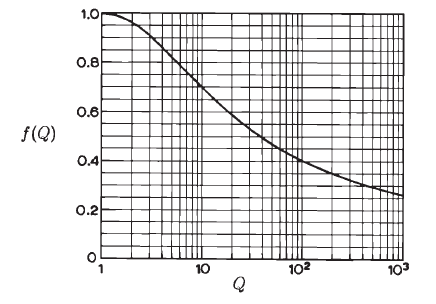
\includegraphics[width=\linewidth]{Abb/f_Q.PNG}
		\caption{Korrekturfunktion der Van-der-Pauw-Methode in Abhängigkeit vom Verhältnis der Widerstände $Q$.}
		\label{f_Q}
	\end{figure}

